\chapter{Bugzilla \\
\small{\textit{-- Spurthi Setty}}
\index{bugzilla} 
\index{Chapter!Bugzilla}
\label{Chapter::Bugzilla}}

\section{Setting Up Bugzilla in Docker on DigitalOcean}

This section documents the detailed procedure for setting up Bugzilla using Docker on a DigitalOcean Ubuntu 22.04 Droplet.  
The setup uses Docker Compose with two services: a MariaDB database and an Apache-based Bugzilla application container.

\subsection{Environment Setup}

\begin{enumerate}
    \item \textbf{Create the Droplet:}  
    - OS: Ubuntu 22.04 LTS  
    - Size: 2 vCPUs, 4 GB RAM (recommended minimum)  
    - Note the public IP address (e.g., \texttt{167.99.54.162}).

    \item \textbf{Update and Install Docker:}

    \begin{minted}[fontsize=\small,breaklines]{bash}
sudo apt update && sudo apt upgrade -y
sudo apt install docker.io docker-compose -y
sudo systemctl enable docker
sudo systemctl start docker
docker --version
docker compose version
    \end{minted}

    \item \textbf{Verify Docker Installation:}

    \begin{minted}[fontsize=\small,breaklines]{bash}
docker --version
docker compose version
    \end{minted}
\end{enumerate}

\subsection{Deploying Bugzilla via Docker Compose}

\begin{enumerate}
    \item \textbf{Create Directory Structure:}

    \begin{minted}[fontsize=\small,breaklines]{bash}
mkdir -p /opt/bugzilla
cd /opt/bugzilla
    \end{minted}

    \item \textbf{Create the Docker Compose File:}

    \begin{minted}[fontsize=\small,breaklines]{yaml}
version: '3'
services:
  db:
    image: mariadb:10.6
    restart: always
    environment:
      MYSQL_ROOT_PASSWORD: root
      MYSQL_DATABASE: bugzilla
      MYSQL_USER: bugs
      MYSQL_PASSWORD: bugs
    volumes:
      - bugzilla_db_data:/var/lib/mysql

  bugzilla:
    image: bugzilla/bugzilla-dev:latest
    restart: always
    ports:
      - "8080:80"
    depends_on:
      - db
    volumes:
      - bugzilla_data:/var/www/html/bugzilla

volumes:
  bugzilla_db_data:
  bugzilla_data:
    \end{minted}

    \item \textbf{Start the Containers:}

    \begin{minted}[fontsize=\small,breaklines]{bash}
docker compose up -d
docker ps
    \end{minted}

    The Bugzilla service listens on port \texttt{8080} on the host, mapped to port \texttt{80} inside the container.
\end{enumerate}

\subsection{Configuring Bugzilla Inside the Container}

\begin{enumerate}
    \item \textbf{Access the Running Container:}

    \begin{minted}[fontsize=\small,breaklines]{bash}
docker exec -it bugzilla-bugzilla-1 bash
    \end{minted}

    \item \textbf{Create and Configure the Database:}

    \begin{minted}[fontsize=\small,breaklines]{bash}
mysql -uroot -e "CREATE DATABASE IF NOT EXISTS bugzilla CHARACTER SET utf8mb4;"
mysql -uroot -e "CREATE USER 'bugs'@'localhost' IDENTIFIED BY 'bugs';"
mysql -uroot -e "GRANT ALL PRIVILEGES ON bugzilla.* TO 'bugs'@'localhost'; FLUSH PRIVILEGES;"
    \end{minted}

    \item \textbf{Set Up Bugzilla Configuration:}

    \begin{minted}[fontsize=\small,breaklines]{bash}
cd /var/www/html/bugzilla
cat > localconfig <<'CONF'
$db_driver = 'mysql';
$db_host   = 'localhost';
$db_name   = 'bugzilla';
$db_user   = 'bugs';
$db_pass   = 'bugs';
$webservergroup = 'apache';
$urlbase = 'http://167.99.54.162:8080/bugzilla/';
CONF
chown -R apache:apache .
    \end{minted}

    \item \textbf{Initialize Bugzilla:}

    \begin{minted}[fontsize=\small,breaklines]{bash}
perl checksetup.pl
    \end{minted}

    The script validates Perl modules, initializes the database schema, and generates the \texttt{params.json} configuration file.
\end{enumerate}

\subsection{Resolving Apache Configuration and Permissions}

\begin{enumerate}
    \item \textbf{Fix Permissions:}

    \begin{minted}[fontsize=\small,breaklines]{bash}
chown -R apache:apache /var/www/html/bugzilla
chmod -R 755 /var/www/html/bugzilla
    \end{minted}

    \item \textbf{Replace the Default Apache Configuration:}

    \begin{minted}[fontsize=\small,breaklines]{bash}
rm -f /etc/httpd/conf.d/welcome.conf
cat >/etc/httpd/conf.d/bugzilla-root.conf <<'CONF'
ServerName 127.0.0.1
DocumentRoot "/var/www/html/bugzilla"

<Directory "/var/www/html/bugzilla">
    Options +ExecCGI +FollowSymLinks
    AllowOverride All
    Require all granted
    AddHandler cgi-script .cgi
</Directory>

DirectoryIndex index.cgi
CONF
    \end{minted}

    \item \textbf{Restart Apache (no systemd available):}

    \begin{minted}[fontsize=\small,breaklines]{bash}
pkill -f httpd || true
/usr/sbin/httpd -DFOREGROUND &
    \end{minted}
\end{enumerate}

\subsection{Testing and Verification}

\begin{enumerate}
    \item \textbf{Verify Local Connectivity:}

    \begin{minted}[fontsize=\small,breaklines]{bash}
curl -I http://127.0.0.1/bugzilla/
    \end{minted}

    Expect either \texttt{HTTP/1.1 200 OK} or \texttt{302 Found (index.cgi)}.

    \item \textbf{Verify Host Mapping:}

    \begin{minted}[fontsize=\small,breaklines]{bash}
curl -I http://127.0.0.1:8080/
    \end{minted}

    \item \textbf{Access the Web Interface:}

    \begin{minted}[fontsize=\small,breaklines]{bash}
http://167.99.54.162:8080/
    \end{minted}

    Log in with:
    \begin{verbatim}
    admin@example.com / admin123
    \end{verbatim}
\end{enumerate}

\subsection{Troubleshooting Notes}

\begin{itemize}
    \item \textbf{403 Forbidden Error:}  
    Fixed by defining explicit \texttt{Require all granted} and enabling CGI execution in Apache config.

    \item \textbf{500 Internal Server Error:}  
    Caused by missing \texttt{params.json}; running \texttt{perl checksetup.pl} regenerates it.

    \item \textbf{Apache Startup Errors:}  
    If logs are missing, recreate them:
    \begin{minted}[fontsize=\small,breaklines]{bash}
mkdir -p /var/log/httpd
touch /var/log/httpd/error_log /var/log/httpd/access_log
chown -R apache:apache /var/log/httpd
    \end{minted}

    \item \textbf{Testing Without Browser:}  
    Use:
    \begin{minted}[fontsize=\small,breaklines]{bash}
curl -I http://127.0.0.1/bugzilla/
    \end{minted}
\end{itemize}

\subsection{Final Result}

Bugzilla was successfully deployed and is accessible at:

\begin{center}
\textbf{\url{http://167.99.54.162:8080/}}
\end{center}
\begin{figure}
    \centering
    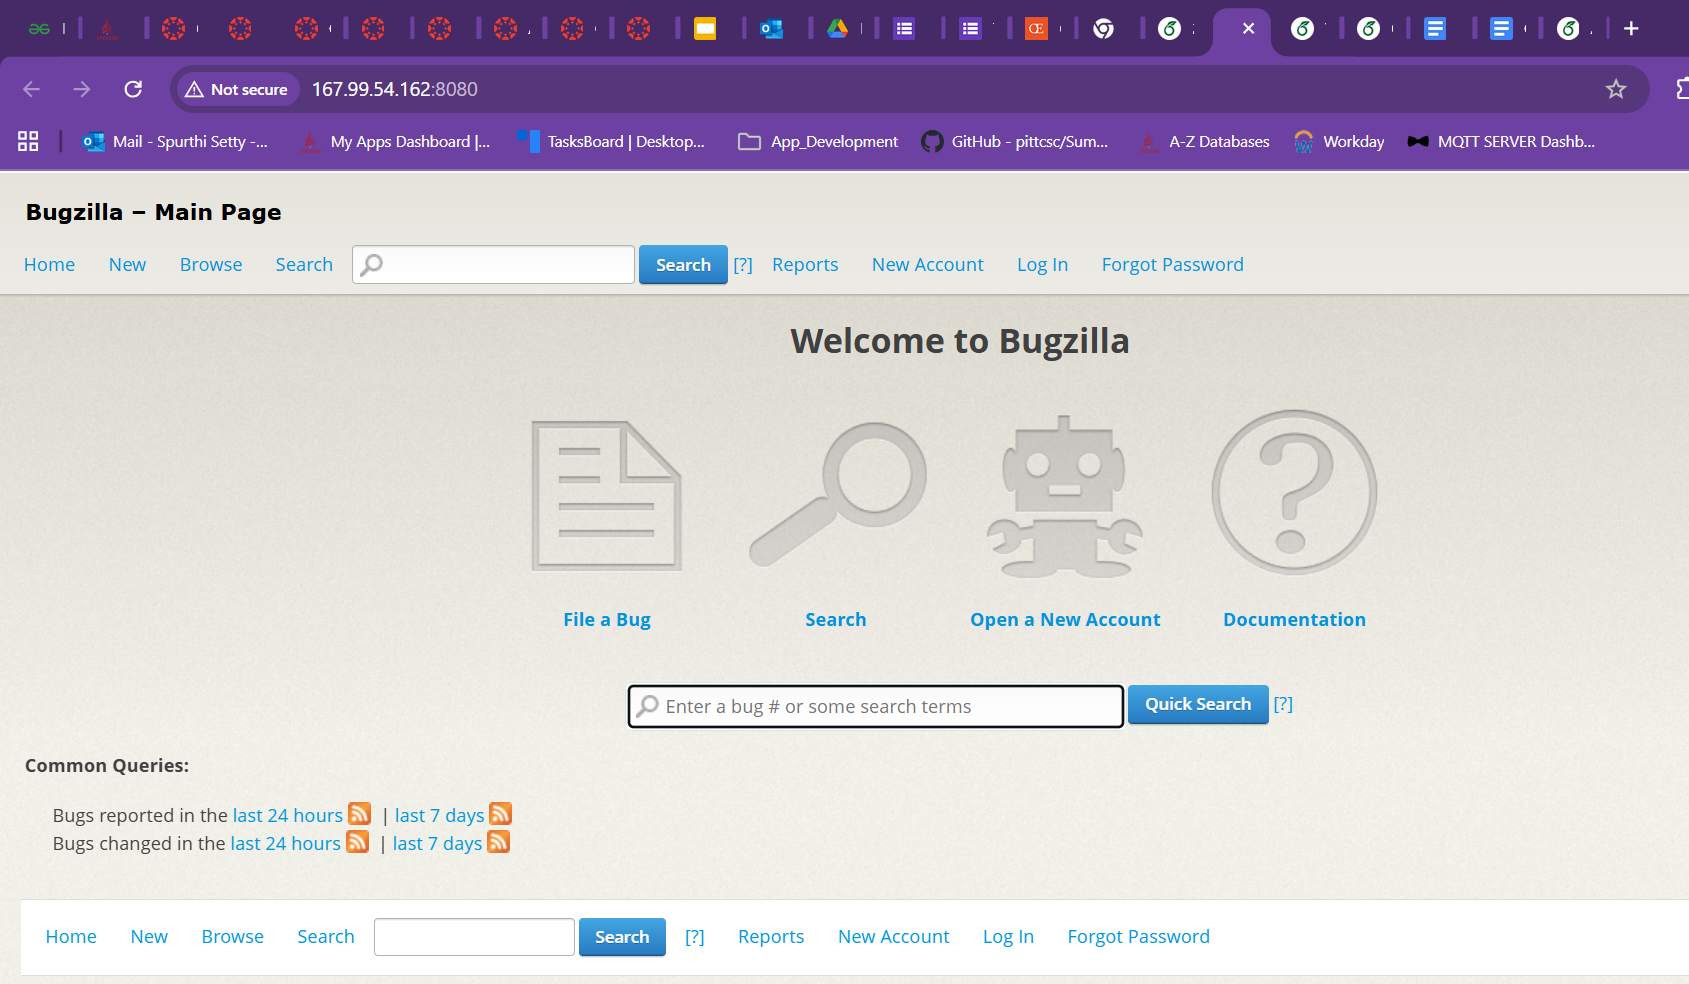
\includegraphics[width=0.7\linewidth]{png/bugzilla.png}
    \caption{Screenshot of bugzilla working at \url{http://167.99.54.162:8080/} }
    \label{fig:placeholder}
\end{figure}
This configuration persists through container restarts, with all data stored in Docker volumes defined in the Compose file.
